
In Abbildung \ref{fig:Schaltbild} wird der Gleichstrommotor des Umwuchtsystems, vereinfacht durch das physikalische Modell einer Nebenschlussmaschine dargestellt. Diese besteht aus einem Wicklungssystem des Ankerkreises und einer Erregerwicklung, welche dem Motor parallel geschaltet ist. Aufgrund von Wicklungen und Streufeldern im Ankerkreis entsteht eine Induktivität $L_A$, über welche die Spannung $U_L$ abfällt. Dazu ist ein Widerstand $R_A$ geschaltet. Der Gleichstrommotor wird dabei ausschließlich von der Klemmspannung $U$ gesteuert. \\

\begin{figure}[!hbt]
	\centering
	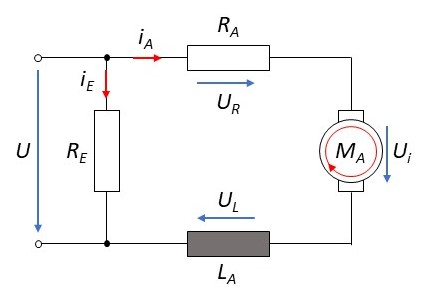
\includegraphics[width=0.5\linewidth]{Images/ProjektB_Elektrik_Ph_Modell_Schaltplan}
	\caption{Physikalisches Modell mit Spannungen und Strömen}
	\label{fig:Schaltbild}
\end{figure}

Die gegebenen Systemparameter lauten dabei:

\begin{table}[!hbt]
	\centering
	
	\begin{tabular}{| l | l |}
		\hline
		Ankerflussverkettung, Motorkonstante & $M_A = 50 \frac{\newton\meter}{\ampere}$ \\
		\hline
		Ohmscher Widerstand des Ankerkreises & $R_A = 0.1 \ohm$ \\
		\hline
		Induktiver Widerstand des Ankerkreises & $L_A = 10 \frac{\volt\second}{\ampere} = 10 \henry$ \\
		\hline
		Klemmspannung & $U = 100 \volt$ \\
		\hline
	\end{tabular}
\captionabove{Systemparameter des physikalischen Modells}
\label{tab:SystemparameterPH}
\end{table}


Aufgrund der Schaltung in Abbildung \ref{fig:Schaltbild} und der Vernachlässigung des Erregerstroms $i_E$, ergibt sich das mathematische Modell der Nebenschlussmaschine mit den drei Systemgleichungen des Unwuchtsystems:

\begin{equation}
\begin{aligned}
&U = U_R + U_i + U_L \\
&U = R_A i_A + K_A \dot{\varphi} + L_A \frac{\diff{i_A}}{\diff{t}} \\
\frac{\diff{i_A}}{\diff{t}} &= \frac{1}{L_A} (U - K_A \dot{\varphi} - i_A R_A) = f_1(U, \dot{\varphi}, i_A)
\end{aligned}
\end{equation}

Translatorisch:

\begin{equation}
\begin{aligned}
(m_1 + m_2) \ddot{s} - m_2 e(\ddot{\varphi} \sin{\varphi} + \ddot{\varphi^2} \cos{\varphi}) + d_t \dot{s} + c s &= 0 \\
\ddot{s} = \frac{1}{m_1 + m_2}[m_2 e(\ddot{\varphi} \sin{\varphi} + \ddot{\varphi^2} \cos{\varphi}) - d_t \dot{s} - c s] &= f_2(\varphi, \dot{\varphi}, \ddot{\varphi}, s, \dot{s}) \label{enq:Bewgltrans}
\end{aligned}
\end{equation}

Rotatorisch:

\begin{equation}
\begin{aligned}
m_2 e^2 \dot{\varphi} - m_2 e \sin{\varphi} (\ddot{s} + g) d_r \dot{\varphi} - M_A &= 0 \\
m_2 e^2 \dot{\varphi} - m_2 e \sin{\varphi} (\ddot{s} + g) d_r \dot{\varphi} - K_A i_A &= 0 \\
\ddot{\varphi} = \frac{1}{m_2 e^2} [m_2 e \sin{\varphi} (\ddot{s} + g) d_r \dot{\varphi} + K_A i_A] &= f_3(\varphi, \dot{\varphi}, \ddot{s}, i_A) \label{enq:Bewglrot}
\end{aligned}
\end{equation}

%Folgesituationen
\begin{figure}[hbt]
	\begin{tikzpicture}
	
	%Zeichnung de Holzblöcke
	\draw (4,0.5) rectangle (9,2.5) node[midway, align=center](Block){Unwuchtsystem}; 
	
	%Pfeile
	\begin{scope}
	\draw[->] (0,1.5) -- (4,1.5);
	\draw[->] (9,1.5) -- (13,1.5);
	\end{scope}
	
	%Parameterbeschriftungen
	\draw(0,2.25) node(uin) {$u = U$};
	\draw(13.75,2.25) node(yvek) {$\underline{y} = \left[\begin{array}{c} s \\\ \dot{\varphi} \\\ M_A \\\ F_U \end{array}\right]$};
	
	\end{tikzpicture}
	
	%Abbildungsunterschrift
	\caption{Unwuchtsystem mit Eingangsspannung und Ausgang (Kinematik, Kinetik)}
	\label{fig:Unwuchtsystem}
	
\end{figure}

Die gegebenen mechanischen Systemparameter lauten dabei:

\begin{table}[!hbt]
	\centering
	
	\begin{tabular}{| l | l |}
		\hline
		Massen & $m_1 = 90 \kilogram \text{; } m_2 = 10 \kilogram$ \\
		\hline
		Federkonstante & $c = 1600 \frac{\newton}{\meter}$ \\
		\hline
		Dämpfungskonstanten & $d_t = 5 \frac{\newton\second}{\meter}$ \\
		\hline
		Rotationsarm & $e = 0.2 \meter$ \\
		\hline
		Erdbeschleunigung & $g = 9.81 \frac{\meter}{\second^2}$ \\
		\hline
	\end{tabular}
	\captionabove{Systemparameter des mechanischen Modells}
	\label{tab:SystemparameterME}
\end{table}

\begin{figure}[hbt]
	\centering
	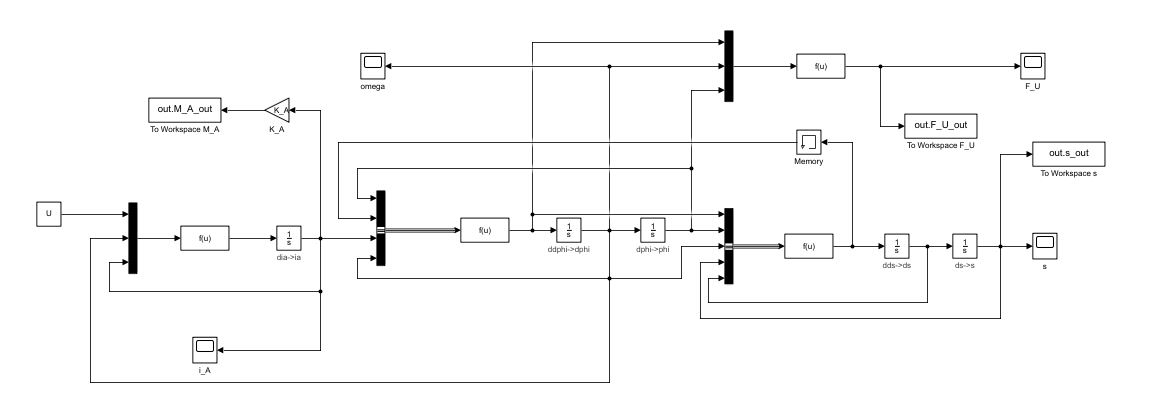
\includegraphics[width=1\linewidth]{Images/ProjektB_Elektrik_Blockdiagramm}
	\caption{SIMULINK Blockdiagramm zur Simulation des Systemverhaltens mit Memory-Block zur Umgehung der algebraischen Schleife}
	\label{fig:Blockdiagramm}
\end{figure}

\begin{figure}[hbt]
	\centering
	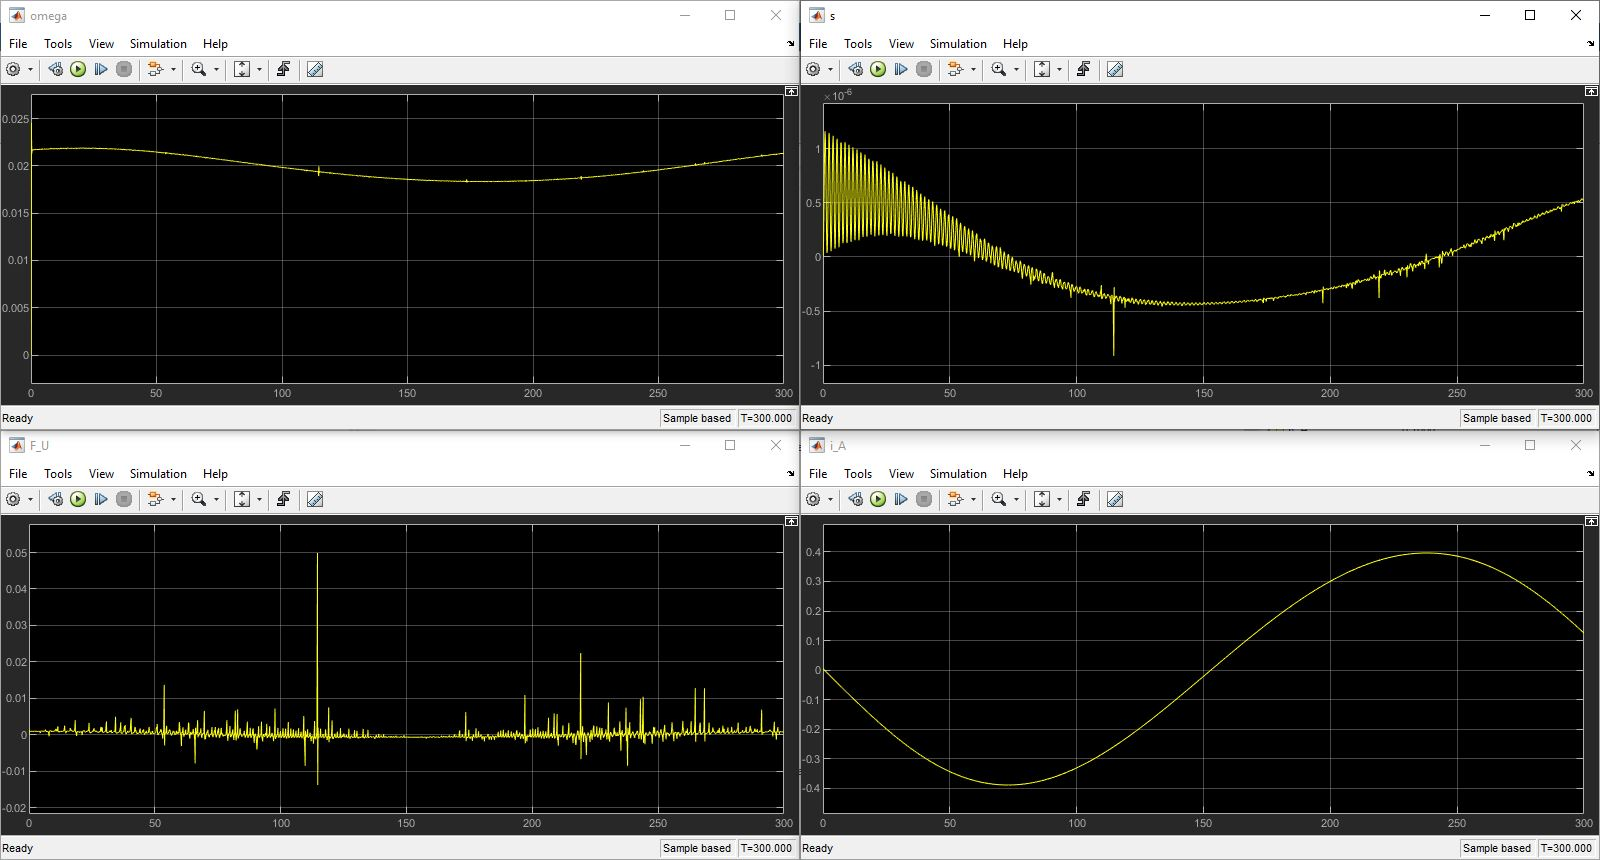
\includegraphics[width=0.5\linewidth]{Images/ProjektB_Elektrik_Diagramme_1}
	\caption{Simulationsergebnisse}
	\label{fig:Simulationsergebnisse}
\end{figure}
